\section{Algorithme approch\'e sur des graphes}

\subsection{Exemple pour 2 approch\'e}

Soit \textit{G} un graphe tel qu'il n'existe qu'une seule feuille. Par
cons\'equent chaque noeud ne poss\`ede qu'un seul et unique fils. Nous
prendrons un arbre de ce type mais de taille 3.

Si nous appliquons l'algorithme vu en cours nous obtiendrons une
couverture optimale, et si nous appliquons notre algorithme nous
obtiendrons une couverture deux fois plus grande que la couverture optimale.


\bigskip


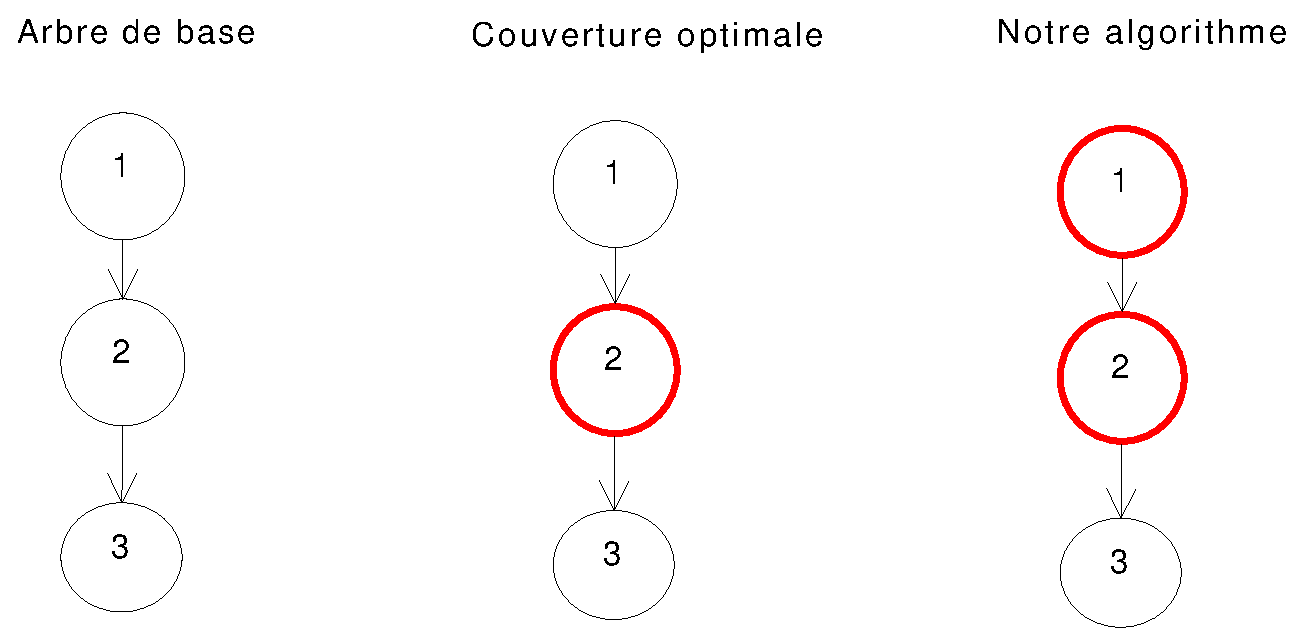
\includegraphics[width=15cm]{arbredoublecouverture}

Nous avons orient\'e le graphe pour donner un sens \`a notre arbre,
mais notre arbre n'est pas orient\'e.\\
On constate que nous prenons les noeuds 1 et 2, alors que l'algorithme
de couverture optimale ne prend que le noeud 2. Nous avons donc 2 fois
plus de noeuds dans notre couverture que l'algorithme optimale, c'est
donc une couverture 2 approch\'e.

\subsection{Peuve pour 2 approch\'e}

\subsubsection{Preuve par r\'ecursivit\'e pour 2 Approch\'e dans un arbre}

Soit G un arbre de taille n. Soit k le nombre de feuille de notre
arbre G.

On note O, la taille de la couverture optimale et A la taille de la couverture retourn\'e par notre algorithme.

\bigskip
\begin{enumerate}
 \item Pour k = 1,\\


Si notre arbre n'a qu'une seule feuille, alors chaque noeud n'a qu'un
seul fils. Avec notre algorithme nous prendrons n-1 sommets (car k
= 1).\\
Avec l'algo optimal nous avons deux cas possibles :
\begin{itemize}
      	\item $\frac{(n - 1)}{2}$ si n $\equiv$ 1(2),\\
		 car tous les noeuds de la couverture couvrent chacun deux ar\^etes.\\
	\item $\frac{(n)}{2}$ si n $\equiv$ 0(2),\\
		car tous les noeuds de la couverture couvrent chacun deux ar\^etes mais une ar\^ete est couvert deux fois.
\end{itemize}

\bigskip
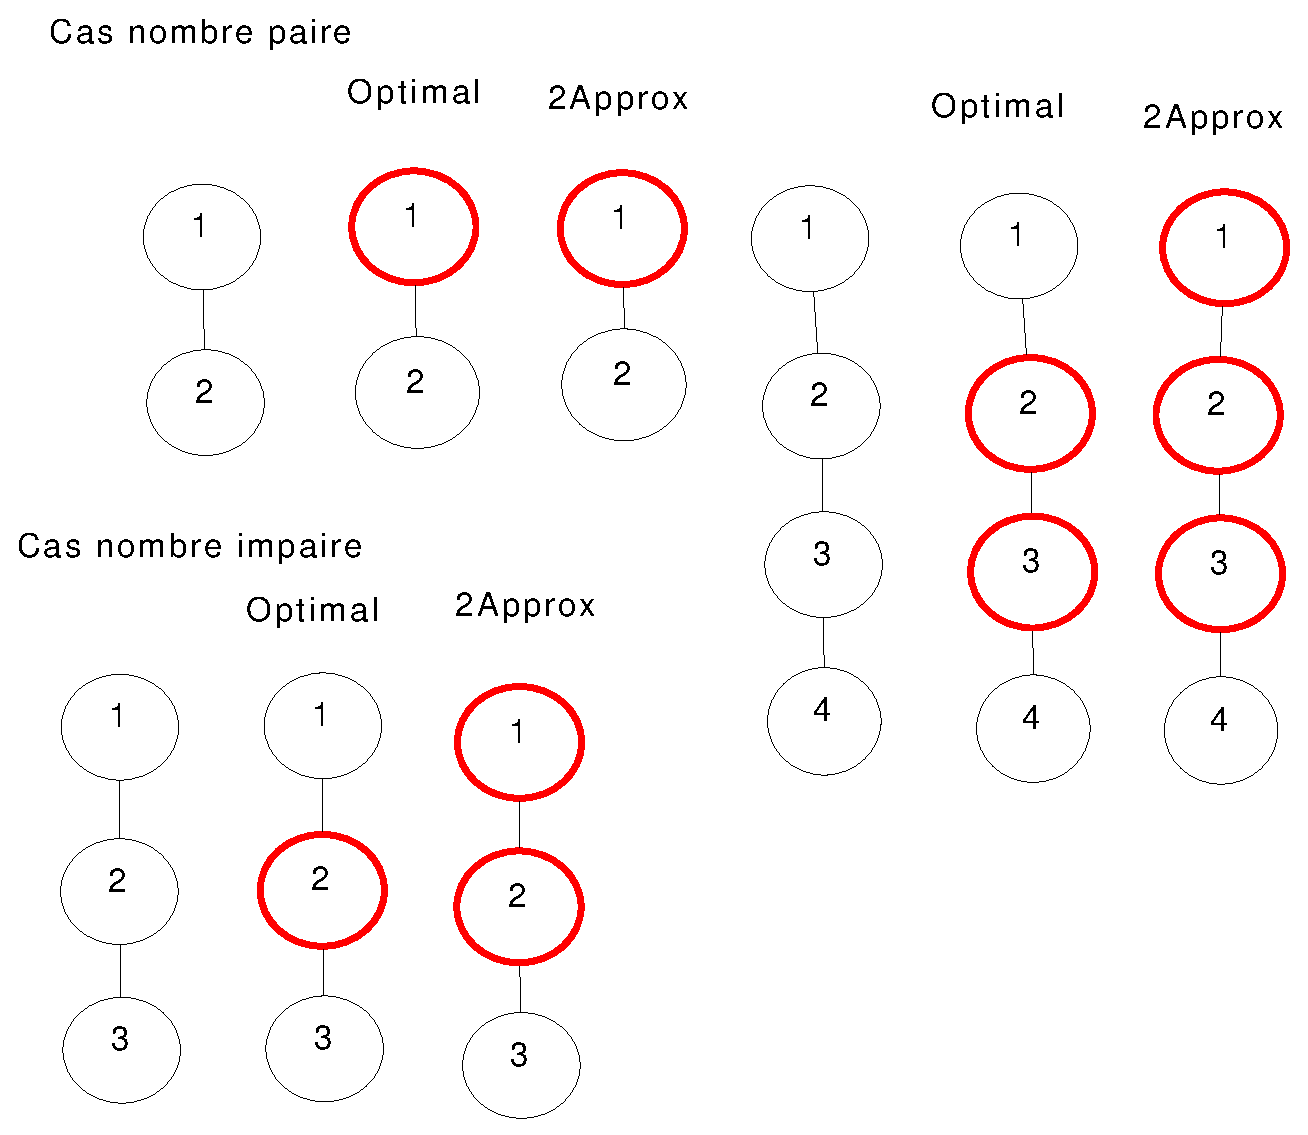
\includegraphics[width=15cm]{demo1}

Donc O  * 2 $\geq$ A.

\item On propose d'admettre que ce cas est vrai, autrement dit que O  * 2 $\geq$ A pour k fils, pour le m\^eme nombre de noeuds (rang n). 

\item Montrons que cela est vrai pour k+1 fils, pour le m\^eme nombre de noeuds.\\

On obtient le graphe suivant :\\

\bigskip
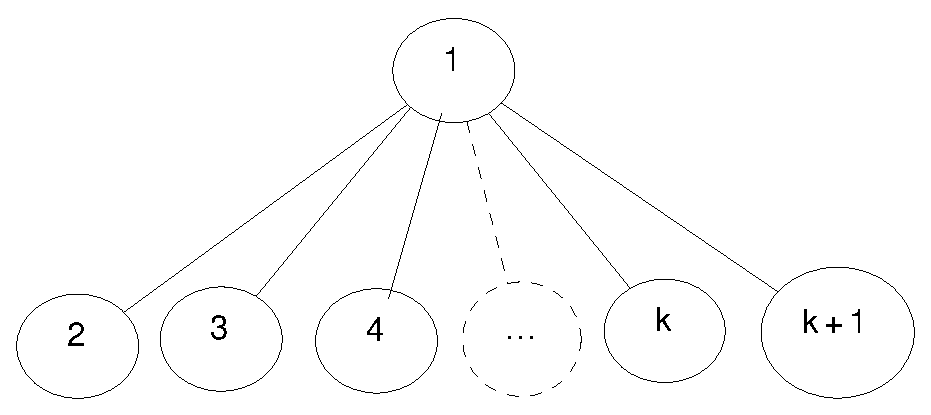
\includegraphics[width=10cm]{demo2}\\

\bigskip
Nous avons un noeud p\`ere et tous les autres sont des racines. Notre couverture optimale est de la m\^eme taille que la couverture de notre algo. Donc O  * 2 $\geq$ A vrai pour tous les arbres.

\end{enumerate}

\subsubsection{Preuve par r\'ecursivit\'e pour 2 Approch\'e dans un graphe}

Soit G un graphe de taille n poss\'edant $\frac{(n(n-1))}{2}$ ar\^etes. Le graphe G est donc fortement connexe.
On note k, le nombre d'ar\^ete que l'on enl\`eve a notre graphe qui restera connexe (mais pas fortement connexe).

\bigskip
\begin{enumerate}
 \item Pour k = 0,\\
Alors nous avons une clique. Notre parcours en profondeur nous retournera un arbre avec une seule feuille. \\
D'apr\`es la preuve pr\'ec\'edente A = n-1 et O = n-1 \'egalement. Donc O * 2 $\geq$ A est vrai

\item On propose d'admettre que cela est vrai jusqu'au rang k = $\frac{(n-1)}{2}$. Il est important de noter que notre graphe doit rester connexe, peu importe sa forme.

\item Montrons que cela est vrai pour k = $\frac{n}{2}$.\\
Nous obtenons donc un graphe de taille n et poss\'edant n-1 ar\^etes. Notre graphe est connexe par cons\'equent, cela est un arbre de taille n. Nous avons d\'ej\`a fait la preuve que O * 2 $\geq$ A pour un arbre de taille n dans la preuve pr\'ec\'edente. Donc cela veut dire que notre preuve est termin\'ee et que O * 2 $\geq$ A.

\end{enumerate}
